\documentclass[12pt,letterpaper,notitlepage]{article}
% Authors: Computational Physics Zoltan Papp & Andreas Bill
% A few introductory LaTeX remarks:
% There are many documents on the internet for an introduction to LaTeX. But you may be able to start with
% those commentaries I wrote below.
% The % sign is for commentaries in a latex document. All what follows the % on a line does not appear in the
% compiled document.
% You need to compile the program to see the text in postscript or pdf format. For that LaTeX must be installed on
% your system. It is free and is often installed when you have a Linux/Unix system.
% Every command starts with a backslash \
% Two backslashes \\ means : new line. You can also write \newline.
% Every mathematical expression (subscripts, vectors, etc.) is either contained between two $ signs (for example 
% $x_1$ if it is in the text, or between the commands
% \begin{eqnarray}
% x_1
% \end{eqnarray}
% Certain symbols such as & { } are used as commands in text and tables and have a predefined meaning. If you 
% want to have it in the text, you simply need to put a backslash in front of it: \&. This is in particular true for the curly
% brackets {} because they are used to define command: \begin{eqnarray}.
% The line on top of this document always needs to be the first line of the LaTeX document. You can change style by
% replacing "article" with "report", "book", etc.
% If you want the American Physical Society Journals standard Physical Review (Letters, A, B, C,...) then you write instead
% of the expression above the following (for prb = Phys.Rev.B):
% \documentclass[aps,prb,floatfix]{revtex4}

% A LaTeX file contains packages allowing to do certain operations. For example the first below allows to draw 
% graphics both BW and containing colors. The second allows to have .eps figures implemented. etc...
\usepackage{color,graphicx}
\usepackage{epsfig,epsf}
\usepackage{epstopdf}
\usepackage{curves}
\usepackage{hyperref}
\usepackage{caption}
\usepackage{tabularx}
\usepackage{graphicx}
\usepackage{pbox}
\usepackage{pdflscape}
\usepackage{bbold}
% The following packages are important as they allow to write certain mathematical expressions.
\usepackage{amsmath}
\usepackage{amssymb}
% To write a code in a LaTeX document you need:
\usepackage{listings}
\usepackage{float}

% Below are typical commands that you may need/want to use for the page dimensions. You can play around, but  
% you don't need it if you use "revtex4" as documentclass.
%\tolerance=10000
%\textwidth18cm
%\textheight24cm
%\oddsidemargin-.5cm
%\topmargin-2cm
%\parindent4ex
%\pagestyle{empty}
%\markright{Test thisl \hfill command!} %Look at the top of the second page when you test it!...

% You can define aliases for long commands. I often do so as shown below, although Physical Review does not 
% accept them. But it is not difficult to replace the new command by the standard one. Here a few of those I use often:
%
%% Own definitions:
\newcommand{\BEq}{\begin{eqnarray}}
\newcommand{\EEq}{\end{eqnarray}}
\newcommand{\BEqn}{\begin{eqnarray*}}
\newcommand{\EEqn}{\end{eqnarray*}}
%% The above first command for example means that instead of writing 
%% \begin{eqnarray}
%% to start an equation and can simply write
%% \BEq
%% The star in the third and fourth commands mean that you write an equation but don't number it.
%% The command \begin{equation} also exists, but allows to write only one single line of equation.
%% With the command \begin{eqnarray} you can write several lines of equations, each line delimited from the other 
%% by the new line symbol \\. You can also align the equations by choosing what sign should be aligned in each line
%% (for example the = sign) and write &=&. Note you can write the &=& only once per line!
%
%% When one wants Eqs(1a,1b,1c) etc. then use \BEqM ... \EEqM or the sequence \BM \BEq ... \EEq \EM:
\newcommand{\BM}{\begin{subequations}}
\newcommand{\EM}{\end{subequations}}
\newcommand{\BEqM}{\begin{subequations}\begin{eqnarray}}
\newcommand{\EEqM}{\end{eqnarray}\end{subequations}}
\newcommand{\Bitem}{\begin{itemize}}
\newcommand{\Eitem}{\end{itemize}}
\newcommand{\Ben}{\begin{enumerate}}
\newcommand{\Een}{\end{enumerate}}
%% Greek letters:
\renewcommand{\a}{\alpha}
\renewcommand{\b}{\beta}
\newcommand{\D}{\Delta}
%%
%% Colors:
% e.g.: \TB{text} will write "text" in color blue.
\newcommand{\TB}[1]{\textcolor{blue}{#1}}
\newcommand{\TR}[1]{\textcolor{red}{#1}}

\newcommand{\bm}[1]{\mbox{\boldmath $#1$}}
\newcommand{\non}{\nonumber\\}

%% Some simplified expressions:
\def\eps{\varepsilon}
\def\r{\right}
\def\l{\left}
\def\p{\partial}
\def\d{\delta}
\newcommand{\ta}{\mbox{$\theta$}}
\newcommand{\ve}{\mbox{${\cal E}$}}
\newcommand{\etab}{\bar{\eta}}
\newcommand{\sg}{\tilde{\sigma}}
\newcommand{\tap}{\mbox{$\theta'$}}
\newcommand{\tta}{\mbox{$\tilde{\theta}$}}
\newcommand{\ttap}{\mbox{$\tilde{\theta}'$}}
\newcommand{\taz}{\mbox{$\theta_0$}}
\newcommand{\phip}{\mbox{$\phi'$}}
\newcommand{\tphi}{\mbox{$\tilde{\phi}$}}
\newcommand{\tphip}{\mbox{$\tilde{\phi}'$}}
\newcommand{\ty}{\mbox{$\tilde{y}$}}
\newcommand{\gb}{\mbox{$\bar{\gamma}$}}
\newcommand{\gone}{\mbox{$\gamma_1$}}
\newcommand{\gtwo}{\mbox{$\gamma_2$}}
\newcommand{\phiz}{\mbox{$\phi_0$}}
\newcommand{\Nf}{\mbox{$N_f$}}
\newcommand{\Nv}{\mbox{$N_v$}}
\newcommand{\qt}{\mbox{$\tilde{q}$}}
\newcommand{\qa}{\mbox{$q_\alpha$}}
\newcommand{\tqa}{\mbox{$\tilde{q}_\alpha$}}
\newcommand{\dqa}{\mbox{$\delta q_\alpha$}}
\newcommand{\pqa}{\mbox{$\partial_{u} q_\alpha$}}
\newcommand{\pqta}{\mbox{$\partial_{u} \tilde{q}_\alpha$}}
\newcommand{\pdqa}{\mbox{$\partial_{u}\delta q_\alpha$}}
\newcommand{\sn}{\mbox{${\rm sn}$}}
\newcommand{\cn}{\mbox{${\rm cn}$}}
\newcommand{\dn}{\mbox{${\rm dn}$}}
\newcommand{\cd}{\mbox{${\rm cd}$}}
%%% Creation, destruction operators:
\newcommand{\cks}{\mbox{$c_{{\bf k},\sigma}$}}
\newcommand{\cksd}{\mbox{$c_{{\bf k},\sigma}^\dagger$}}
\newcommand{\cku}{\mbox{$c_{{\bf k},\uparrow}$}}
\newcommand{\ckd}{\mbox{$c_{-{\bf k},\downarrow}$}}
\newcommand{\ckud}{\mbox{$c_{{\bf k},\uparrow}^\dagger$}}
\newcommand{\ckdd}{\mbox{$c_{-{\bf k},\downarrow}^\dagger$}}


% That's the actual beginning of the document. All commands above affect the whole text, those below affect the 
%  text locally.
\begin{document}

\lstset{language=Fortran,tabsize=4,numbers=left,numberstyle=\tiny,basicstyle=\ttfamily\small\color{dkblue},stringstyle=\ttfamily\color{blue},keywordstyle=\rmfamily\color{dkred}\bfseries\emph,backgroundcolor=\color{white},commentstyle=\color{dkgreen}}




\title{%
	Final Report   \\
\large Computational Physics - Phys 562}
\author{Benjamin Deutsch  \\
Department of Physics\\
California State University Long Beach}
\date{\today}
\maketitle



\begin{abstract}
No abstract    
\end{abstract}

%%%%%%%%%%%
\section{Problem 1}
\subsection{Method(Description of code)}
For the first question, we notice the separable differential equations, and make use of the Runge Kutta subroutine as given in class. Carefully, we edit the derivative statements {\tt{f(1), f(2), f(3)}} to appear the same as the testing sheet as;
	\begin{equation}
		\frac{dx}{dt}=-(y+z),\hspace{5mm} \frac{dy}{dt}=x+ay, \hspace{5mm} \frac{dz}{dt}=b+z(x-c)
	\end{equation}
It should be noted that we have preserved the calculation for K, as it is fundamental for the RK4 step method. It will be used within the subroutine to adjust the increment of interpolations based on the slope at given interval points.  After this has been done, we must check that the intent in and out statements do match with your written functions, for call by the main routine. 
Within the main routine, we have changed the module to notify the program that we have three equations that will be used externally, as well as the parameters {\tt a, b, c} to be passed into the subroutine as well. The real benefit of the RK subroutine is seen in utilizing a simplified program, here along with parameters {\tt a, b, c} being defined, we have also included time step criteria and initial conditions, all of which will be implemented in the external subroutine. Finally the creation of a do loop cycling over an defined interval of time, calls to the subroutine with the above parameters and writes the output to specific files.  These are then graphed for analysis.  	
\subsection{Results}
In parts A and B of question 1, we were asked to alter certain parameter and investigate the resulting behavior. In order to do this we have altered these variables manually within the code (as guided by the comments). 
The effects of part A, varying {\tt c} from 5 to 8 can be seen below. A few things can be said here, firstly that in lowering the c value to 5 we can see a increasingly repetitive trend in the graph, as bolder lines in specific regions begin to form. Increasing the duration of this value only seems to localize the values, controlling the level of disorder in the system. This is further reinforced by the repetitive nature of the c = 8 graph (right), the spacing of each pathway is distributed almost evenly. Lastly comparing the two time dependent graphs for each set of parameters indicates that as a and b grow it reaches some limit where in c grows exceptionally quickly, spiking and suppressing grow in a and b parameters. This oscillational property has indicates a precise area of chaotic behavior. \\
In the section for B, we are asked to change the initial condition {\tt x, y, z}, doing this by way of three defined sets, beginning at zeros, x at zero while y and z are negative and lastly x and y being positive and z negative. We can easily see the behavior of the zeros starting system in the below time dependent images, concluding that slowly the graphs returned to "normal" behavior after some time. This is reinforced by reviewing the other two initial conditions (0, -,-) and ( +, +, -). Where the graphs seem to differ is within there complete plots (X, Y, Z), It seems here that as the initial conditions are allowed to be separated farther apart numerically, we observe pathway intervals at more diverse separations.    

\begin{landscape}
\thispagestyle{empty}
\begin{table}
\caption{Part 1; Changing Parameter C}
\hspace{-.75in}
  \begin{tabular}{ccc} 
      \parbox[c]{1em}{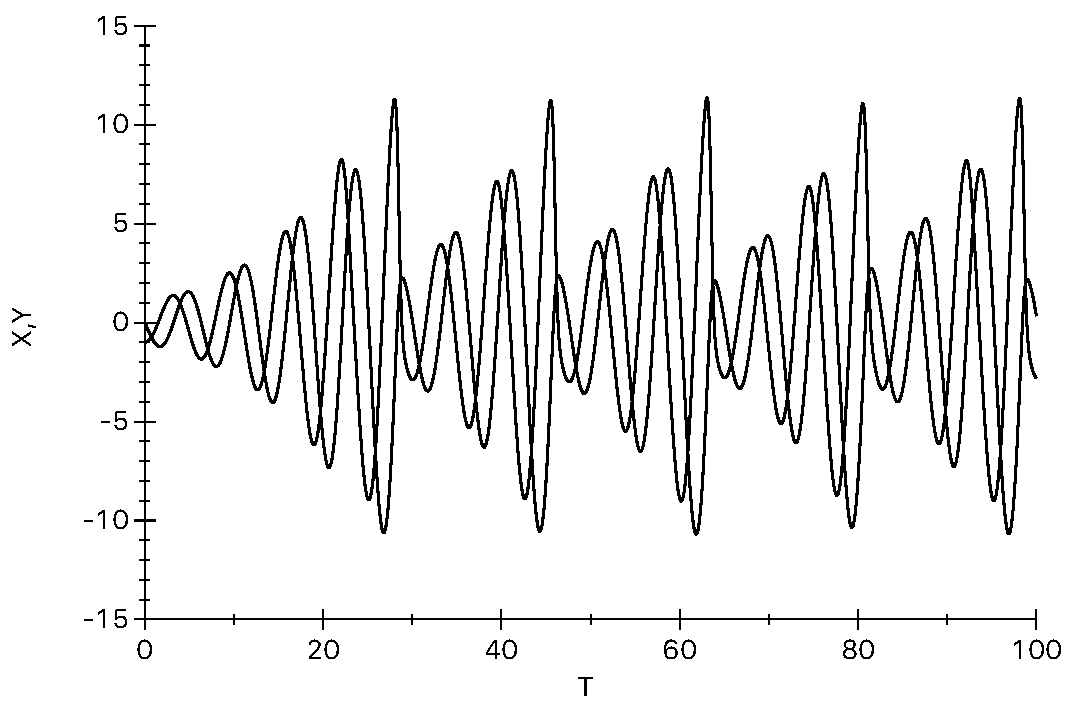
\includegraphics[width=3in]{norm1.pdf}} &
      \hspace{2.5in}       
      \parbox[c]{1em}{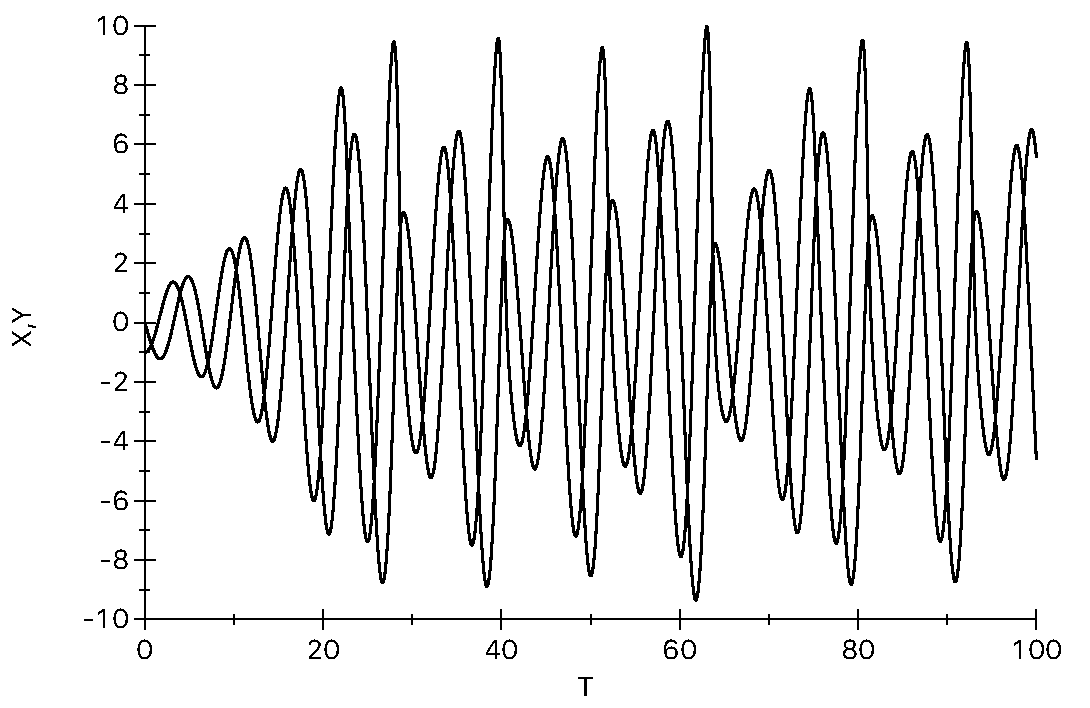
\includegraphics[width=3in]{low1.pdf}} &
      \hspace{2.5in}
        \parbox[c]{1em}{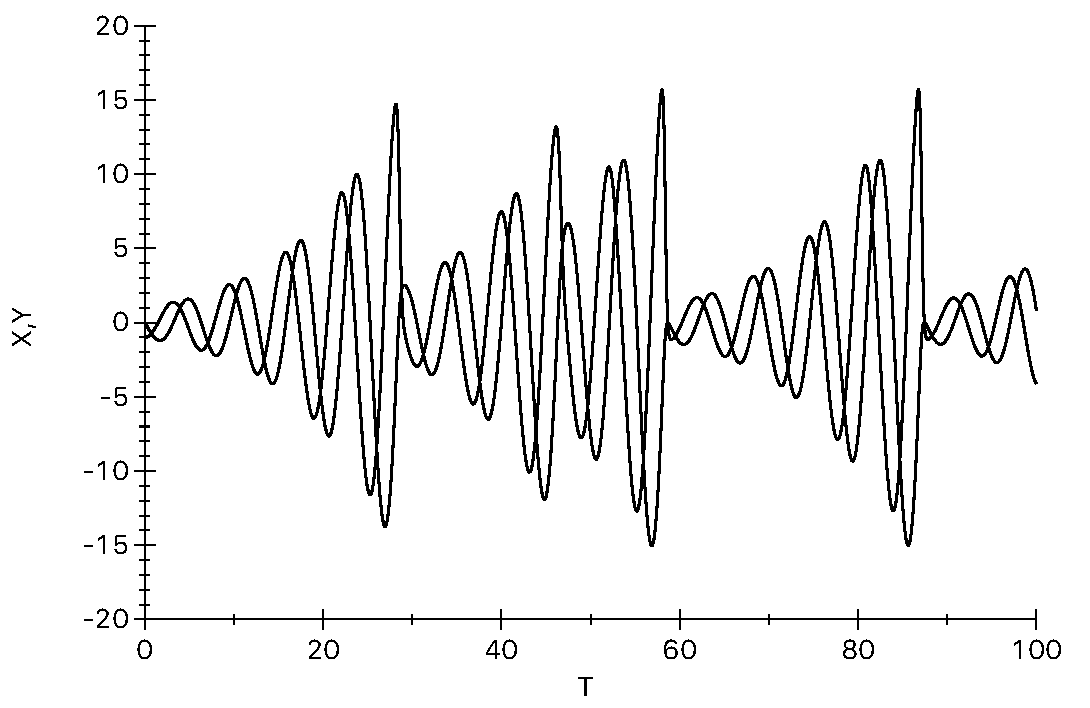
\includegraphics[width=3in]{high1.pdf}} \\
      \parbox[c]{1em}{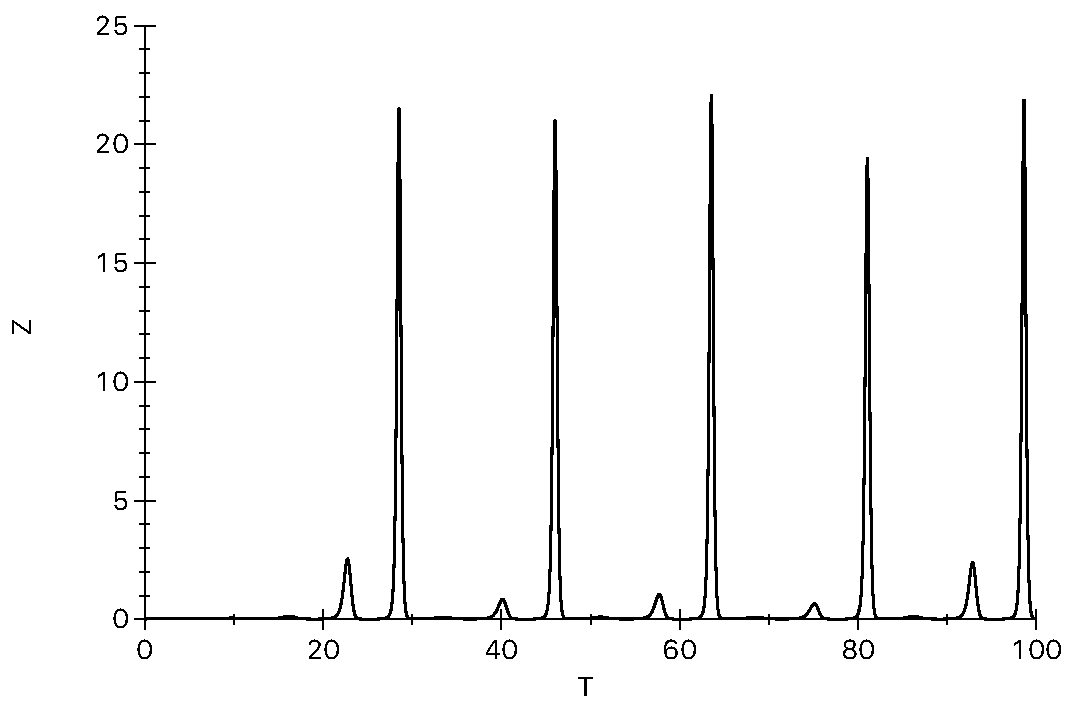
\includegraphics[width=3in]{norm2.pdf}} &
      \hspace{2.5in}
       \parbox[c]{1em}{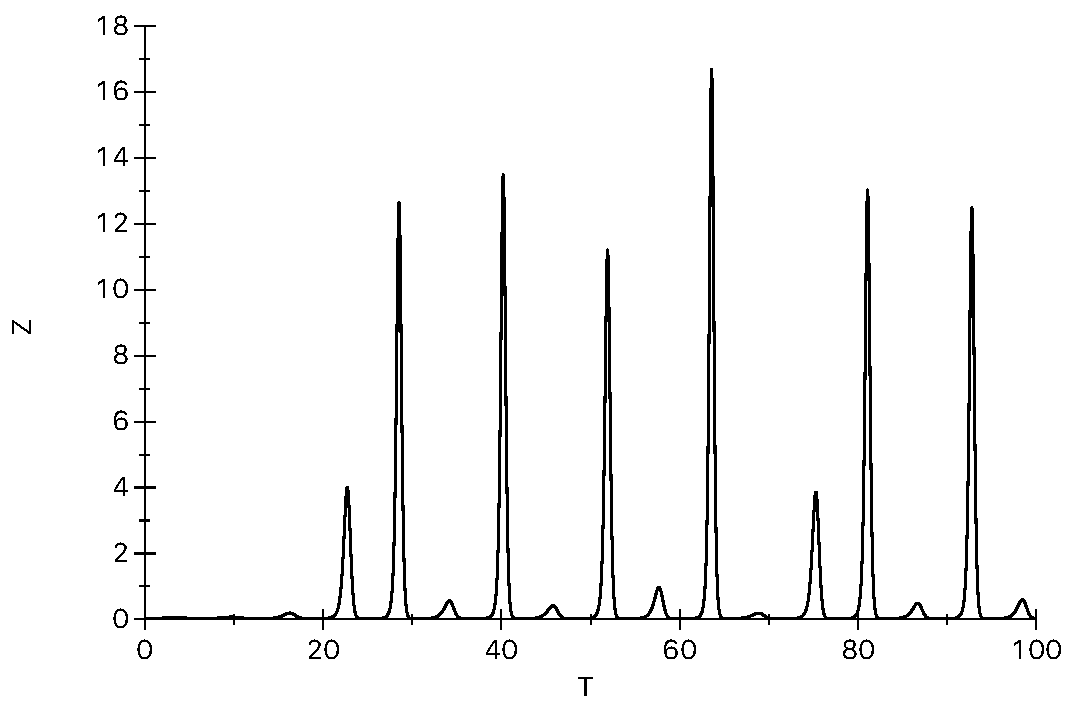
\includegraphics[width=3in]{low2.pdf}} &
       \hspace{2.5in}
        \parbox[c]{1em}{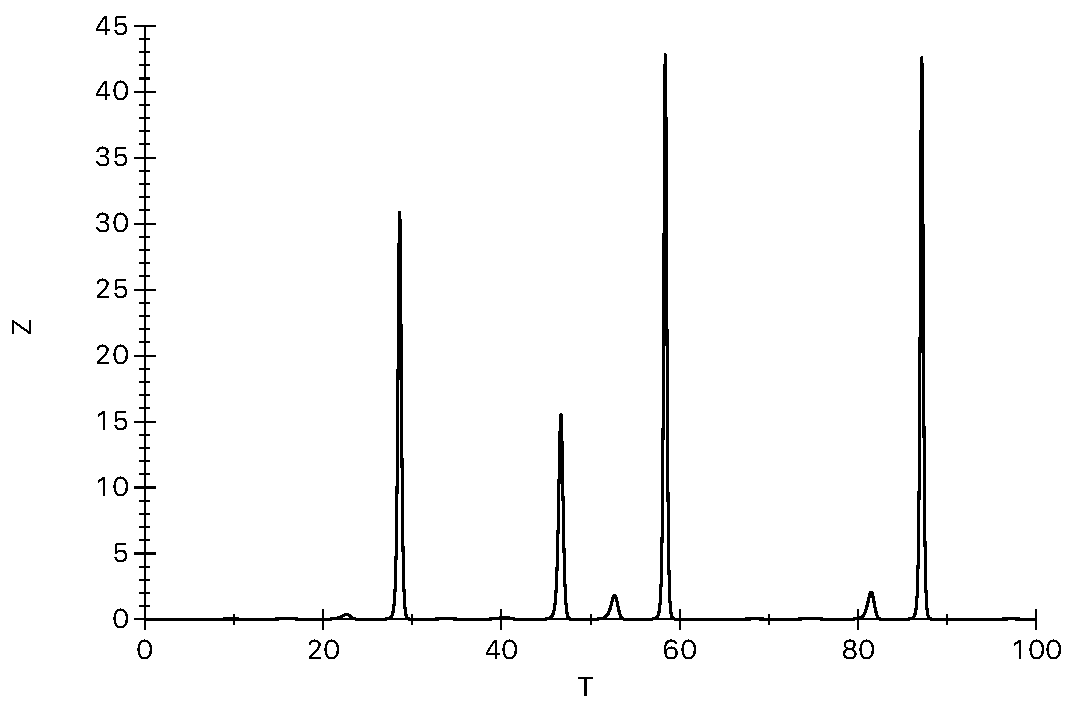
\includegraphics[width=3in]{high2.pdf}} \\
      \parbox[c]{1em}{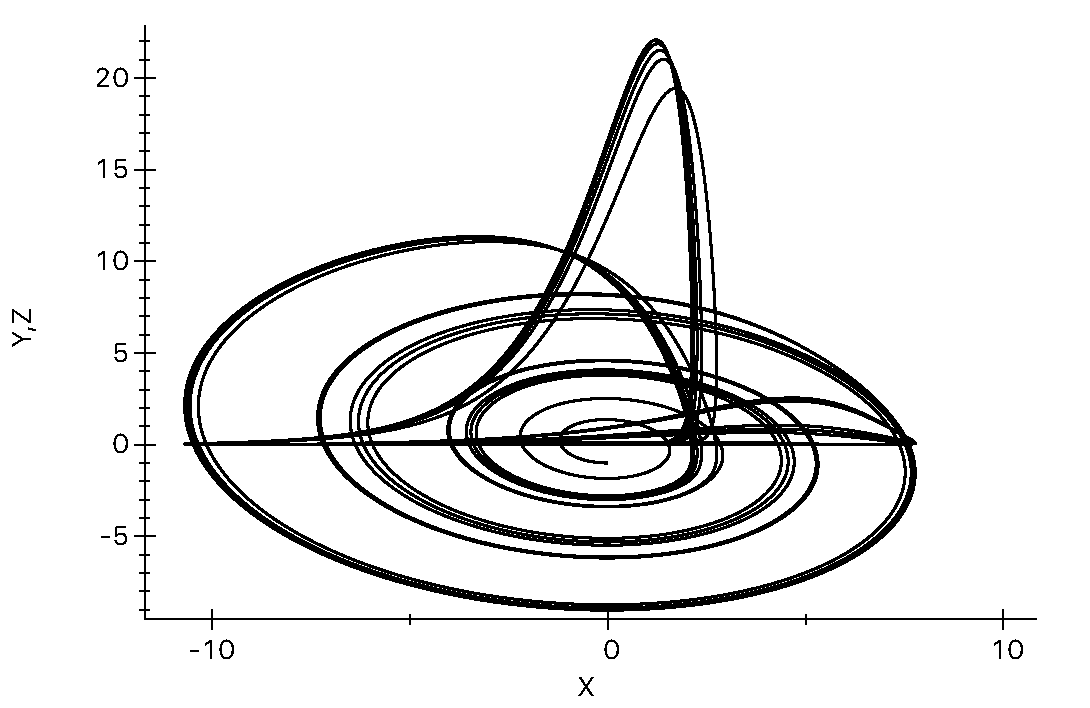
\includegraphics[width=3in]{norm4.pdf}} &
      \hspace{2.5in}
       \parbox[c]{1em}{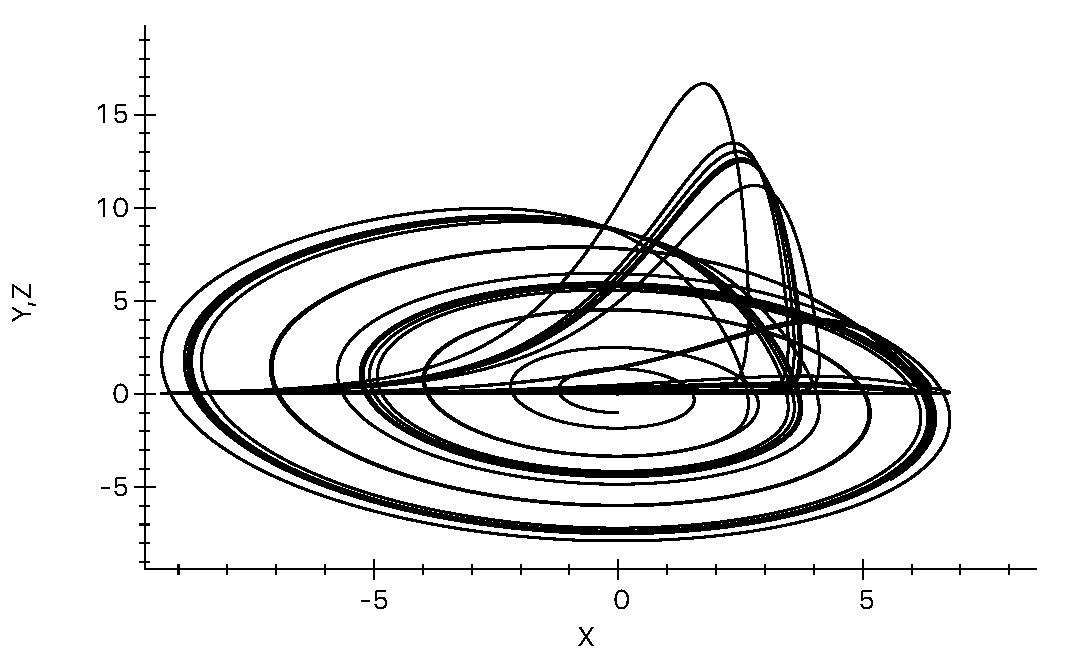
\includegraphics[width=3in]{low4.pdf}} &
       \hspace{2.5in}
        \parbox[c]{1em}{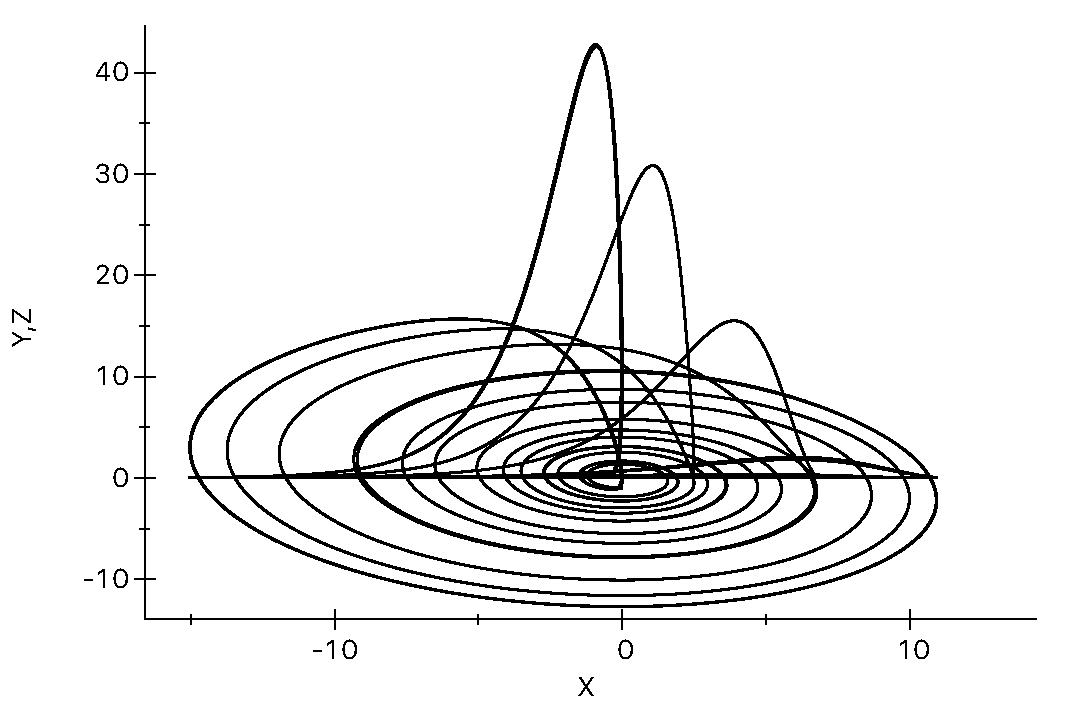
\includegraphics[width=3in]{high4.pdf}} \\  
 \end{tabular}
\end{table}
\end{landscape}

\begin{landscape}
\begin{table}
\caption{Part 2; Initial conditions (000), (0--), (++-)}
\hspace{-.75in}
  \begin{tabular}{ccc} 
      \parbox[c]{1em}{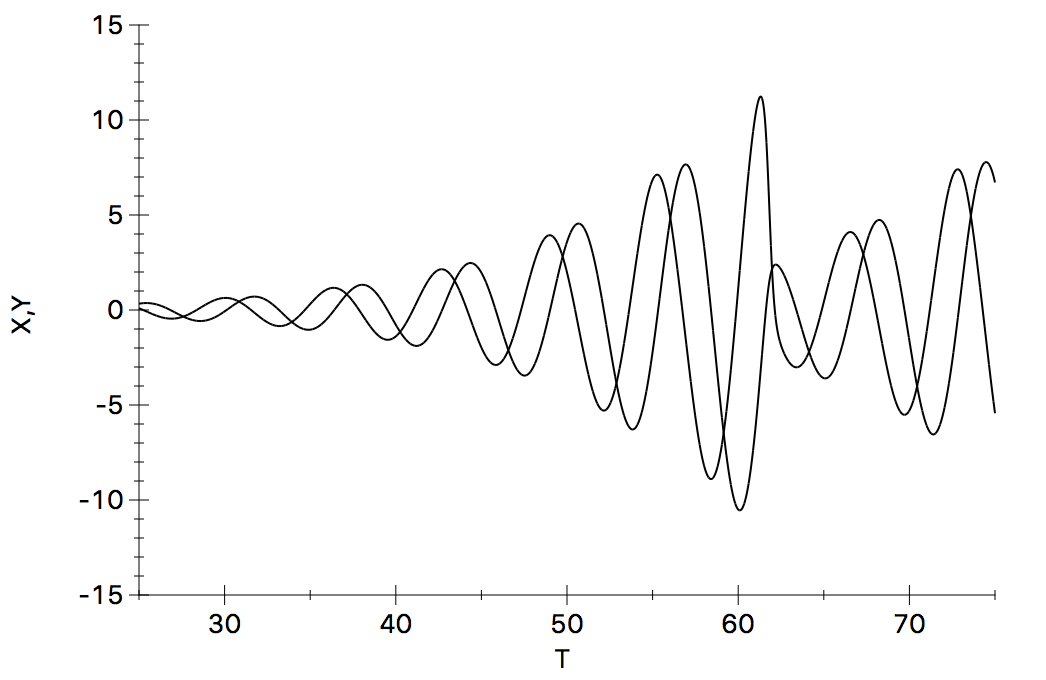
\includegraphics[width=3in]{zerot.png}} &
      \hspace{2.5in}       
      \parbox[c]{1em}{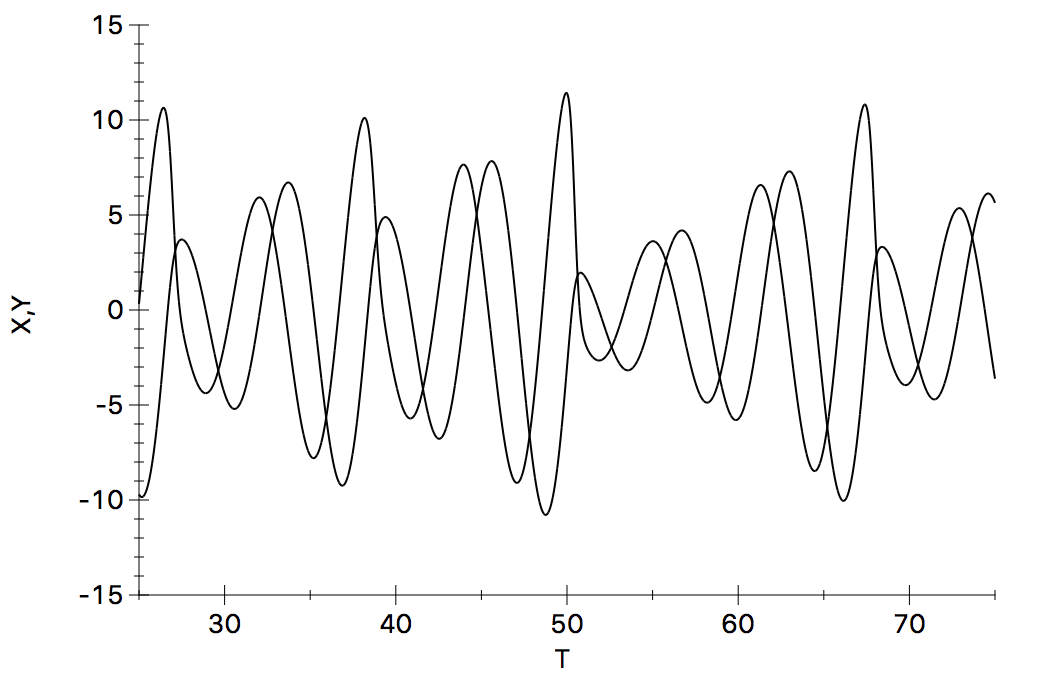
\includegraphics[width=3in]{negt.png}}  &
      \hspace{2.5in} 
       \parbox[c]{1em}{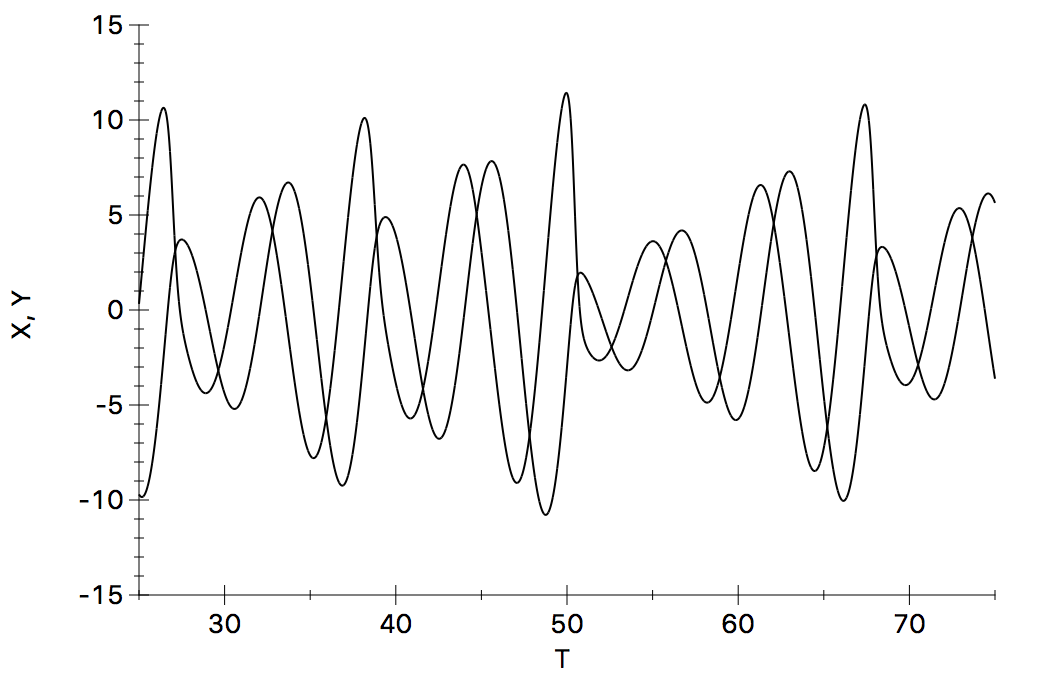
\includegraphics[width=3in]{post.png}}
      \\
 \end{tabular}
\end{table}


\thispagestyle{empty}
\begin{table}
\caption{Part 2; (000), (0--), (++-)}
\hspace{-.75in}
  \begin{tabular}{ccc} 
      \parbox[c]{1em}{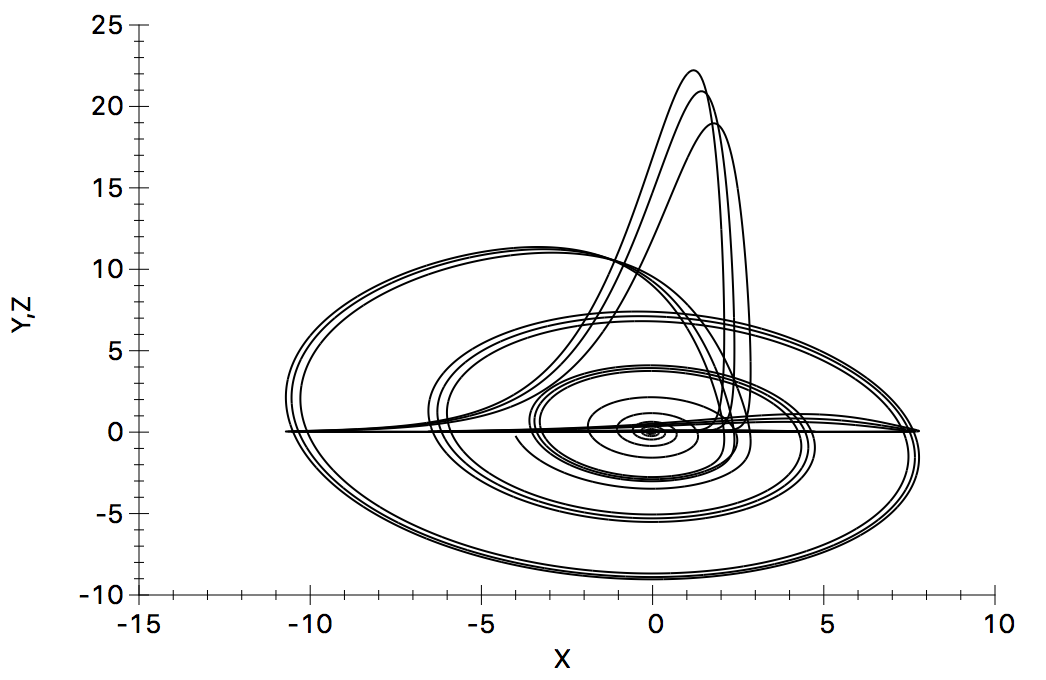
\includegraphics[width=3in]{zerofull.png}} &
      \hspace{2.5in}       
      \parbox[c]{1em}{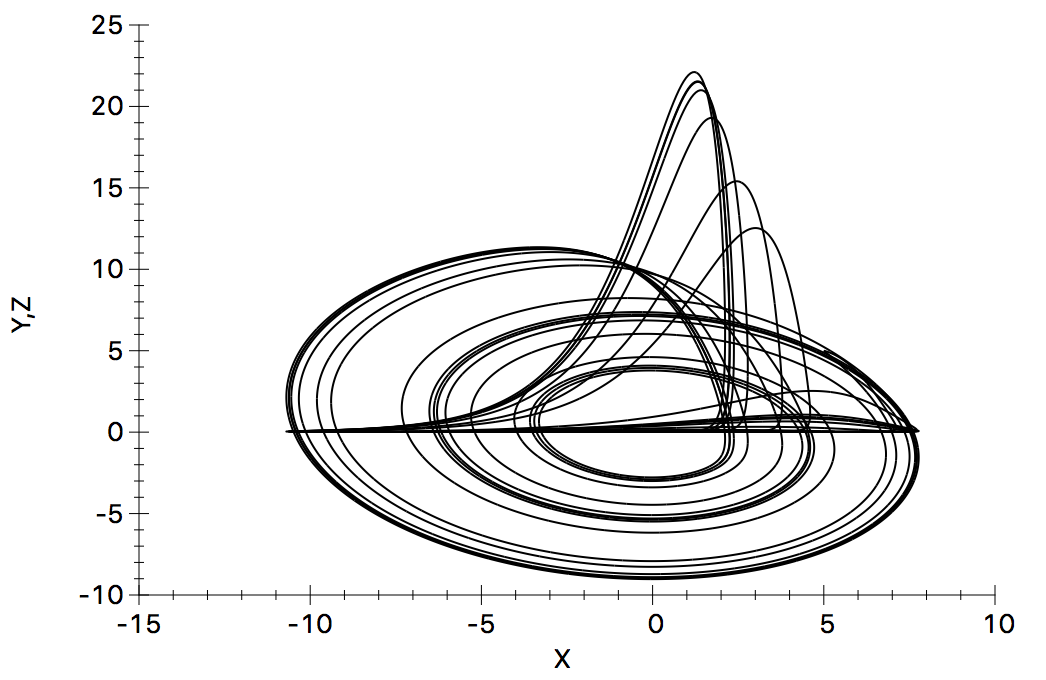
\includegraphics[width=3in]{negfull}} &
      \hspace{2.5in}
        \parbox[c]{1em}{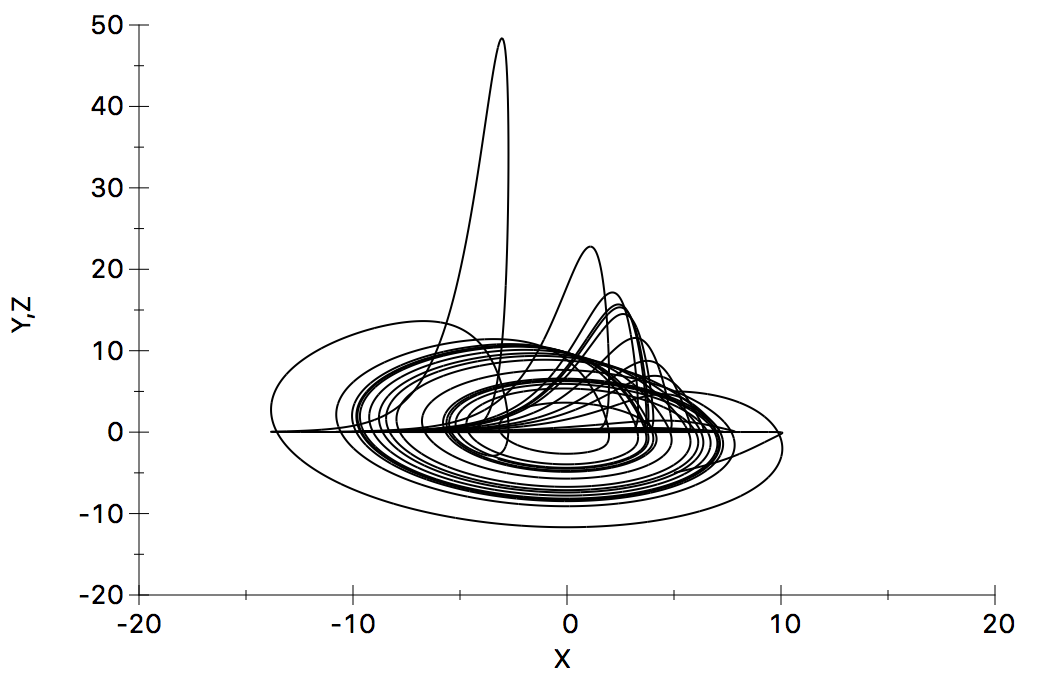
\includegraphics[width=3in]{posfull.png}} \\
 \end{tabular}
\end{table}
\end{landscape}

%%%%%%%%%%
 
\section{Problem 2}
\subsection{Description of code}
To avoid a lengthy discussion on the set up of problem 2, we have utilized past code {\tt Q.f95} (Midterm 4) as a starting point for this code. We can do this for a number of reasons, primarily its purpose was to calculate was to produce a set of eigenvalues and component eigenvectors. It did this, by compiling a working hamiltonian matrix for the 1-D harmonic oscillator. Keys components of the pervious working code utilized,   

	\begin{equation}
		\psi_n(x) = \frac{1}{\sqrt{2^n\,n!}} \cdot \left(\frac{m\omega}{\pi \hbar}\right)^{1/4}\cdot e^{
		- \frac{m\omega x^2}{2 \hbar}} \cdot H_n\left(\sqrt{\frac{m\omega}{\hbar}} x \right)
	\end{equation}   
	
and $\hat{E_n}$ as 
	\begin{equation}
		\hat{E_n}= \left(n+\frac{1}{2}\right) \hbar \omega	
	\end{equation} 
	
to produce (with our oscillator potential) for brevity,

	\begin{equation}
		T_{m,n}=E_{m,n}+U_{m,n}
	\end{equation}
	
and the hamiltonian as;

	\begin{equation}
		H_{m,n}=T_{m,n}+V_{m,n}
	\end{equation} 

Here we are asked to assume a perturbation to the system resulting in changed elements of $H_{0,5}$ and $H_{5,0}$ by $ \frac{\hbar w_H}{2}$ with omega (w2=2).
Simplified we have;

\begin{equation}
		H_p =
					\begin{bmatrix}
					0 		& 0    	& 0 		& 0 		& 1 \\
					0 		& 0 		& 0 		& 0 		& 0 \\
					0 		& 0 		& 0 		& 0 		& 0 \\
					0 		& 0 		& 0 		& 0 		& 0 \\
					1		& 0	        & 0		& 0		& 0 \\
					\end{bmatrix},		
	\end{equation}	
	
With this we can write,

	\begin{equation}
		H_{new}=H_{old}+H_p
	\end{equation}

Part A, Finding the eigenvalues and eigenvector can be easily done here by implementing the {\tt dsyev} subroutine, a component to the LAPACK framework, used to do just this. To check for completeness we have done a little matrix algebra (Fortran's intrinsic {\tt Matmul})  as follows; 
	\begin{equation}
		\mathbb{1}=H_{new}*Transpose(H_{new}) 
	\end{equation}
We have omitted the conjugate in this operation as this is not a complex matrix. 
Achieving the identity we have completed the first task. \\
Part B, was slightly more involved. We are asked to calculate the matrix representation of $ e^{-iHt} $, with H being our newly perturbed matrix. In order to do this, after research it is given that; 
	\begin{equation}
		B=M^{\dagger} * A * M 
	\end{equation}
Where B is your matrix, M are the eigenvalues and A the eigenvectors. So it follows that;
	\begin{equation}
		f(B)=M^{\dagger} * f(A) * M 
	\end{equation}
In order to add this to the main routine, we noticed that since the matrix A (the eigenvalues) needs to contain only diagonal entries we can simply  include the required function e to each individually along with the constants. Finally taking each output and multiplying it against the identity matrix to align the eigenvectors along the diagonals. Note; the matrix while maintaining the dimension of the identity will now be recorded (ZZ matrix) as a complex matrix, due to the multiplication of the i, seen above. \\
Now with a diagonalized matrix of the eigenvalues and a previously computed eigenvector matrix, we can straight forwarding use the equation above (10), and a nested {\tt Matmul} function to produce the final matrix representation. \\
As asked we can alter the t ({\tt tt}) between 1 and 5 manually, as indicated by the comments.
\newpage
\subsection{Results}
\begin {center}
	$\begin{array} {|c|c|}
		\hline
	       & Eigenvalues\\
	       \hline
	   1  &0.57386019704424396\\
	   2  &2.1226186643438076\\
           3  &3.5561285389571826\\
           4  &5.0242884193833461\\
           5  &6.9833016503265242\\
           6  &8.7398024703352171\\
          \hline
      \end{array}$
      \captionof{table}{Eigenvalues for $\omega=2$}
      \end{center}
For results see terminal output.
 \\
These have been compared against Maple software and Wolfram Alpha's Mathematica. 

%%%%%%%%%%%
\section{Problem 3}
\subsection{Description of code}
For problem 3 we are asked to produce a code for calculating the residua for $ f(x)= \pi cot (\pi x ) $ at $x=0$ , $x=0$, and $x=\pi$.
Again we can amend a pervious code in order to fulfill this contour integral, however before doing this we must do a little math.
Given the function;
	\begin{equation}
		f(x)= \frac{\pi}{tan(x)} 	
	\end{equation}
We create the complex contour intergral;
	\begin{equation}
		f(z)= \frac{1}{2\pi}\oint{\frac{\pi}{ tan(\pi z)}} dz \rightarrow   \frac{1}{2i} \oint \frac{1}{tan(\pi z)}
	\end{equation}
Differentiating z
	\begin{equation}
		\frac{1}{2} \int_0 ^{2\pi} \ \frac{1}{tan(\pi * re^{it})} re^{it} dt \hspace{.5cm} = \hspace{.5cm} \frac{1}{2} \int_0 ^{2 \pi} \frac{re^{it}}{tan(\pi * re^{it})} dt
	\end{equation}
With this result we can readily use the {\tt d01bcf} subroutine for calculation of the weights and abscissae needed in approximating  the Gauss-Legendre function type. Through the summation;
	\begin{equation}
		\sum_{i=1} ^{n}	w_i f(x_i)   \hspace{.5cm}  w_i = weights \hspace{.5cm} x_i = abscissae  
	\end{equation}
Here the do loop runs over this sum for our specific problem, held in a external function in order to integrate the resulting residue.  The parameters for which can be changed manually in the code itself, as indicated by the comments.   
\subsection{Results}
The results are as follows, for $f(x)= \frac{\pi}{tan(x)}$
\\\\
\begin{center}
\begin{tabular}{ |c|c| } 
 \hline
 x= 			& f(x)=   \\ 
 \hline
 0 			& 1   \\ 
  $\frac{\pi}{2}$	& 0   \\ 
  $\pi$ 		& 0   \\ 
 \hline
\end{tabular}
\end{center}




%%%%%%%%%%%%
\begin{thebibliography}{}

	\bibitem{}
	Z.~Papp and A.~Bill, {\it Computational Physics Lecture Notes}, California State University Long Beach.
	
\end{thebibliography}



\end{document}
